\scanpage{83}
\mspage{82}
est muni d'un élément \inserted{$\handwritten{\underline}{f}_q$} de $G_{\deleted{a}\handwritten{\nu}}(K_{\deleted{a}\handwritten{\nu}})$\inserted{(\handwritten{``}Frobenius relatif à $\handwritten{\underline}{F}_q$'')}\handwritten{\begin{tikzpicture}[baseline=0cm,x=1cm,y=1cm]\draw[thin] (0,-.15)..controls (-.08,.1) and (.1,.18)..(.23,.18)--(3.5,.18)..controls (3.6,.17) and (3.7,.28)..(3.66,.38);\end{tikzpicture}}. Ce dernier n'est autre d'ailleurs que $\deleted{\handwritten{\underline}{f}_q}$ $\handwritten{\underline}{f}^{\deleted{a}\handwritten{\nu}}$, où $\handwritten{\underline}{f}$ est le générateur canonique de $G$ (le Frobenius \unsure{\rlap{l}a|\rlap{d}a}bsolu \handwritten{!}). \deleted{\unsure{O|C} on voit donc que $G_a$ est encore engendré par} Notons que $a\operatorname{\rlap{i}Id}_G$ est un monomorphis\rlap{e}m\unsure{\rlap{d}e|\rlap{r}e|e} (car $x\handwritten{\mathrel{\begin{tikzpicture}[baseline=-.04cm,x=1cm,y=1cm]\draw[semithick] (0,-.1)--(0,.12) (0,0)--(.55,0) (.55,-.06)--(.55,.06);\end{tikzpicture}}}x^{\deleted{a}\handwritten{\nu}}$ est un épimorphisme dans $\handwritten{\overline}{\handwritten{\underline}{Q}}_{\handwritten{p}}^{\handwritten{*}}$ ), donc \rlap{x}induit un isomorphisme entre $\rlap{$K$}G_{K_{\deleted{a}\handwritten{\nu}}}$ et $G_{\deleted{a}\handwritten{\nu}}\handwritten{\simeq}G(\handwritten{\underline}{F}_q)$,trans\rlap{o}f\rlap{f}ormant le frobenius \deleted{relati} absolu en le frobenius relatif à $\handwritten{\underline}{F}_q$. Grâce à ceci, on voit :

\handwritten{\uline}{Proposition} 10.1. La catégorie \inserted{tann.}\handwritten{\begin{tikzpicture}[baseline=0cm,x=1cm,y=1cm]\draw[thin] (0,-.15)..controls (-.08,.1) and (.1,.18)..(.23,.18)--(0.8,.18)..controls (0.9,.17) and (1.0,.28)..(0.9600000000000001,.38);\end{tikzpicture}} $\operatorname{Fcriso}(\handwritten{\underline}{F}_q)\handwritten{\otimes}_{\overset{\mathrm{Fr.}}{\handwritten{\underline}{Q}}_p}K_a$ est équivalente à la catégorie \inserted{tann.}\handwritten{\begin{tikzpicture}[baseline=0cm,x=1cm,y=1cm]\draw[thin] (0,-.15)..controls (-.08,.1) and (.1,.18)..(.23,.18)--(0.8,.18)..controls (0.9,.17) and (1.0,.28)..(0.9600000000000001,.38);\end{tikzpicture}} $\operatorname{Fcriso}(\handwritten{\underline}{F}_p)\handwritten{\otimes}_{\handwritten{\underline}{Q}_p}K_a$,\handwritten{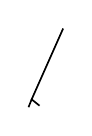
\begin{tikzpicture}[baseline=-.02cm,x=1cm,y=1cm]\draw[semithick] (.4,.9)--(0,0)--(.1,-.08);\draw[semithick] (0,0)--(-.04,-.1);\end{tikzpicture}} \margin{\handwritten{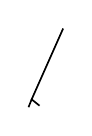
\begin{tikzpicture}[baseline=-.02cm,x=1cm,y=1cm]\draw[semithick] (.4,.9)--(0,0)--(.1,-.08);\draw[semithick] (0,0)--(-.04,-.1);\end{tikzpicture}}\handwritten{i.e. la catégorie des couples $(E,F'_E)$ d'un vectoriel sur $K_\nu$ et d'un autom de ce vectoriel....)}}
avec $\handwritten{\underline}{f}_q$ correspondant à $\handwritten{\underline}{f}^{\deleted{a}\handwritten{\nu}}$ (où on peut, si on veut, considérer $\handwritten{\underline}{f}_q$ et $\handwritten{\underline}{f}$ comme des end\rlap{m}o\unsure{\rlap{E}m|\rlap{h}m|m}orphismes des foncteurs identiques de $\operatorname{Fcriso}(\handwritten{\underline}{F}_q)$ resp. $\operatorname{Fcriso}(\handwritten{\underline}{F}_p)$)), et corres\deleted{p}pondance des foncteurs fibres canoniques. Le foncteur déduit du ch\rlap{n}a\rlap{a}ngement de base $\handwritten{\underline}{F}_p\handwritten{\to}\handwritten{\underline}{F}_q$

\[
\operatorname{Fcriso}(\handwritten{\underline}{F}_{\unsure{\rlap{g}p|\rlap{q}p|p}})\handwritten{\otimes}_{\overset{\mathrm{Fr.}}{\handwritten{\underline}{Q}}_p}K_{\deleted{a}\handwritten{\nu}}\handwritten{\longrightarrow}\operatorname{Fcriso}(\handwritten{\underline}{F}_q)\handwritten{\otimes}_{\handwritten{\underline}{Q}_p}K_{\deleted{a}\handwritten{\nu}}
\]
\unsure{\rlap{n}s|\rlap{e}s|s}'identifie, par l'équivalence précédente, au foncteur qui à tout couple $(E,F_E)$ d'un vectoriel sur $K_{\deleted{a}\handwritten{\nu}}$ et d'un automorphisme dudit, associe le couple $(E,F_E{}^{\deleted{a}\handwritten{\nu}})$\handwritten{;}
\inserted{\handwritten{analogue \unsure{p\textsuperscript{r}|pour} $\operatorname{Fcriso}(F_1)-\operatorname{Fcriso}(F_q)\otimes_{\mathbb{Q}_p}K_\nu$, il s'identifie : $(E,F_E)\longmapsto(E,F_E{}^\nu)$.}}

10.2. Comme on connait $\handwritten{\underline}{G}(\handwritten{\underline}{F}_q)$ comme une sous-gerbe $\handwritten{\underline}{G}_{\deleted{a}\handwritten{\nu}}$ de $\handwritten{\underline}{G}=\handwritten{\underline}{G}(\handwritten{\underline}{F}_p)$, et que celle-ci contient $\handwritten{\underline}{H}$, on connait donc en principe \rlap{d}l'inclusion
\[
\handwritten{\underline}{H}\handwritten{\longrightarrow}\handwritten{\underline}{G}_{\deleted{a}\handwritten{\nu}}=\handwritten{\underline}{G}(F_q)\quad ,
\]
donc aussi le foncteur
\[
\operatorname{Rep}(\handwritten{\underline}{G}_{\deleted{a}\handwritten{\nu}})\handwritten{\simeq}\operatorname{Fcriso}(\handwritten{\underline}{F}_q)\handwritten{\mathrel{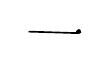
\begin{tikzpicture}[baseline=-.04cm,x=1cm,y=1cm]\draw[semithick] (0,0)--(.65,-.02);\fill (.59,-.02)..controls (.62,.05) and (.67,.05)..(.67,-.02)--cycle;\end{tikzpicture}}}\operatorname{Rep}(\handwritten{\underline}{H})\quad ,
\]
\deleted{\inserted{et} Considérons le foncteur correspondant}
\[
\deleted{\operatorname{\unsure{\rlap{R}F|\rlap{K}F|F}criso}(\handwritten{\underline}{F}_q)\handwritten{\otimes}_{\handwritten{\underline}{Q}_p}K_{\underset{\deleted{a}}{a}}\quad\operatorname{Rep}(\handwritten{\underline}{H})\handwritten{\otimes}_{\handwritten{\underline}{Q}_p}K_a\ .}
\]
\figure{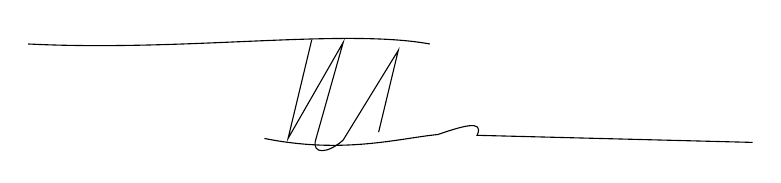
\begin{tikzpicture}[x=1cm,y=1cm]\draw[thin] (0,1.3)..controls (2,1.2) and (4,1.5)..(5.1,1.3);\draw[thin] (3.6,1.35)--(3.3,.1)--(4,1.32)--(3.65,.08)..controls (3.6,-.1) and (3.8,-.1)..(4,.08)--(4.7,1.22)--(4.45,.18);\draw[thin] (3,.1)..controls (4,-.1) and (4.7,.1)..(5.2,.15)..controls (5.5,.25) and (5.8,.35)..(5.7,.14)--(9.2,.05);\end{tikzpicture}}
L'effet de ce\deleted{s} foncteur\deleted{s} sur les classes d'isomorphie d'éléments est connu (comme chaque fois qu'il s'agit d'un morphisme d'une \deleted{gerbe de} \unsure{\rlap{O}c|\rlap{C}c}atégorie tannakienne à lien commutatif dans une autre à lien de type multiplicatif) par la connaiss\rlap{n}a\rlap{a}nee de l'homomorphisme de liens correspondant

